
    %%%%% %%%%% %%%%%
    %               %
    % New row       %
    %               %
    %%%%% %%%%% %%%%%
\begin{columns}[t]
  \begin{column}{0.44\textwidth}
    \begin{block}{\large Rationale}
%\small
\scriptsize
%\tiny
Inference of copy number variation presents a technical challenge because variant callers typically require the copy number of a genome or genomic region to be known a priori.
Our project required us to address this question, so we designed and implemented a method with the following:

\begin{itemize}
\item No a priori known base ploidy is required
\item Allows for genomic windows to be analyzed
\item Flexibility to use with non-model organisms
\item Works with VCF format data
\item Implemented in R
\end{itemize}

We validated these approaches with the model system of \textit{Saccharomyces cerevisiae}, an organism known to vary in ploidy and copy number.
This method has been implemented in the R package vcfR.
\vspace{3mm}
    \end{block}
  \end{column}

  \begin{column}{0.5\textwidth}
    \begin{block}{\large Chromosomal perspectives}
      \begin{columns}
        \begin{column}{0.4\textwidth}
%\small
%\footnotesize
\scriptsize
%\tiny
\\
\vspace{1mm}
%Different data types provide different perspectives.
Sequence depth can be used to characterize base ploidy and deviations from base ploidy.
However, if a research question includes 'what is base ploidy' we need another perspective.
Allele balance can help provide inferences on whether base ploidy is diploid, triploid, or tetraploid.
This is a reproduction of Figure 7 from Zhou et al. (2016) created in vcfR and highlights chromosome XII as having three copies while base ploidy is two copies.
%\vspace{2mm}
%          \begin{figure}
        \end{column}
        \begin{column}{0.55\textwidth}
          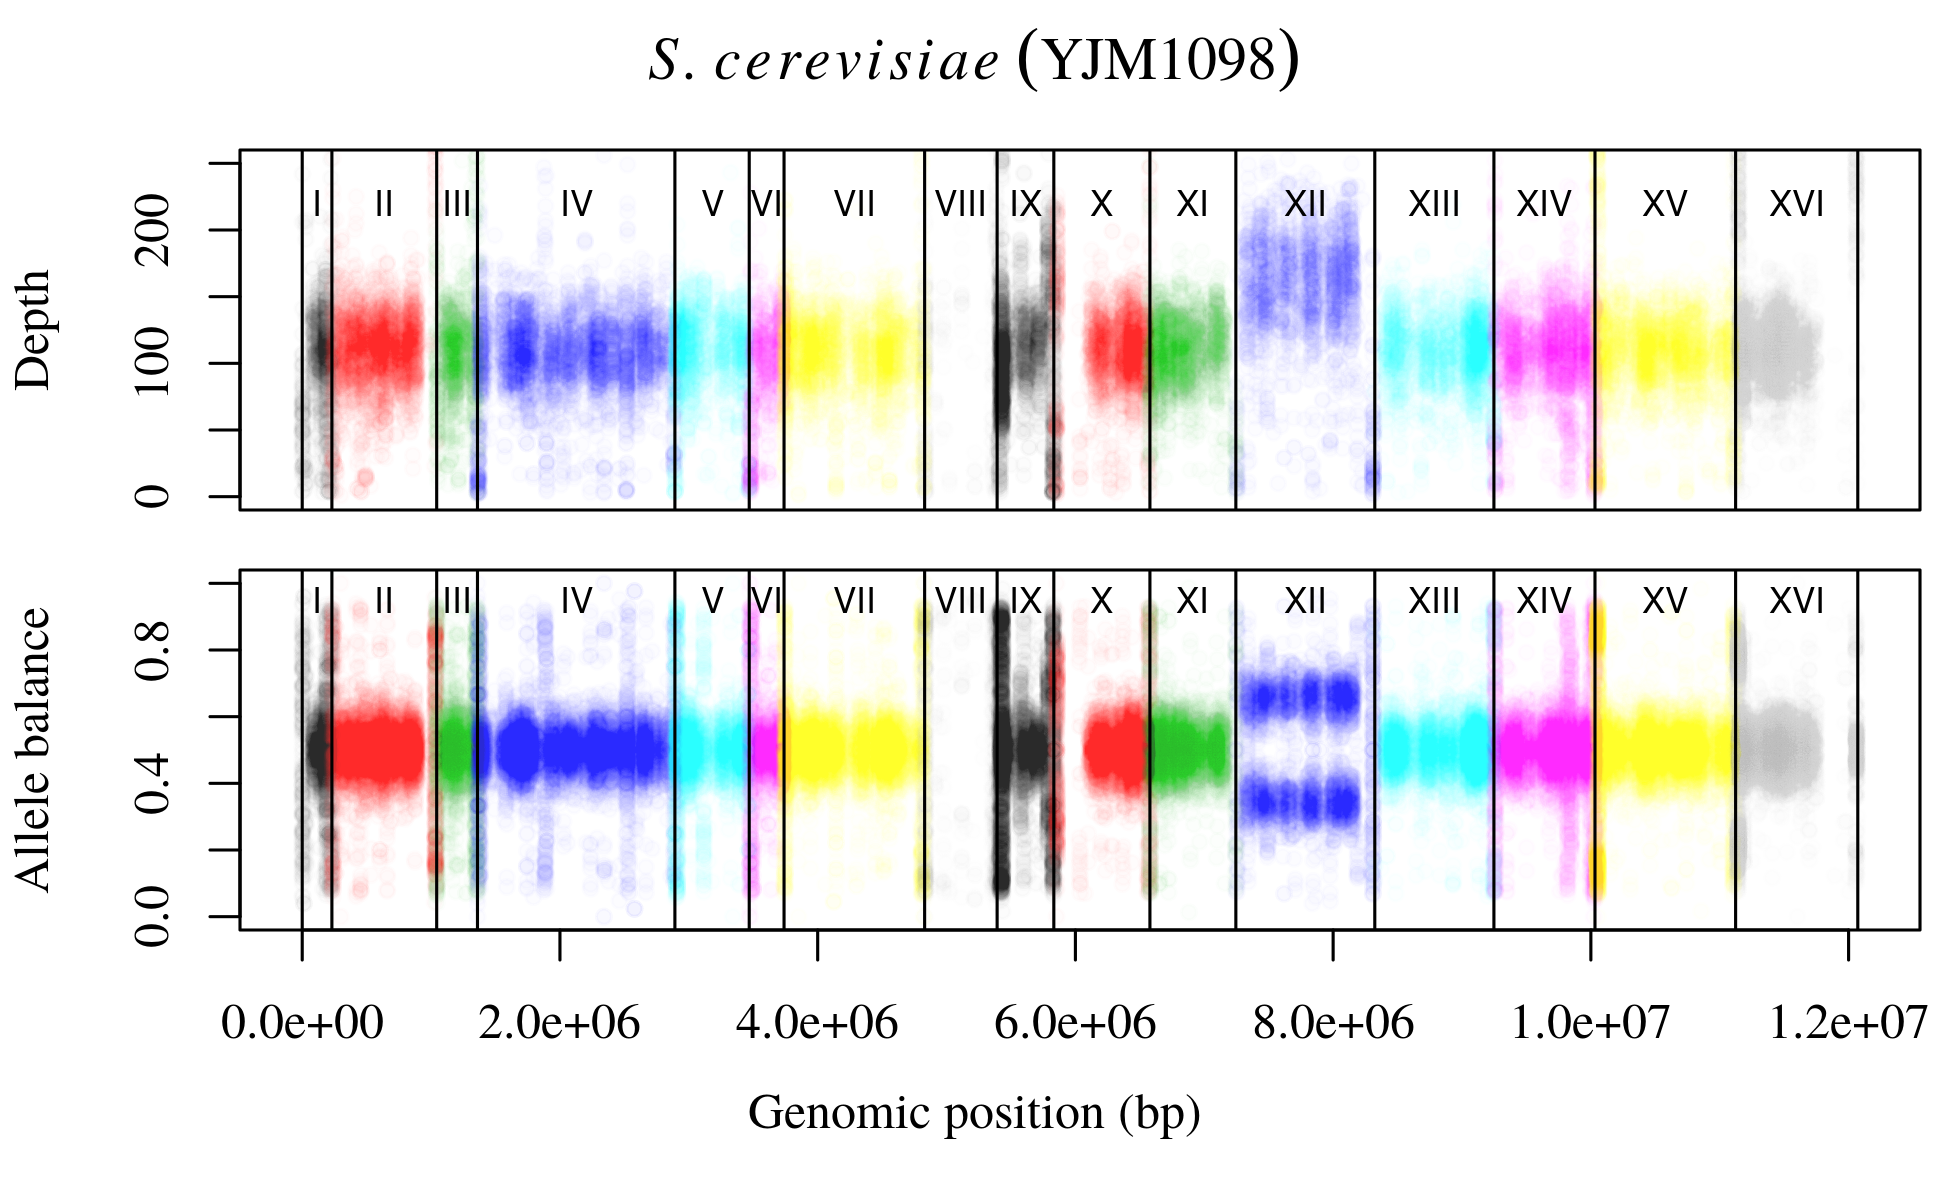
\includegraphics[height=20cm]{./figures/fig4_chrom_YJM1098.png}
        \end{column}
      \end{columns}
%          \caption{Allele balance is the frequency theat the most abundant and second most abundant allele were sequenced at.}
%          \end{figure}

    \end{block}
  \end{column}

\end{columns}


